% ============================================================
\chapter{エントロピー・プーリング}\label{ch:ep}

BL は、市場もビューも正規分布で、ビューは期待リターンの線形の組み合わせ、という枠の中で働く。実際には、リターンの分布は裾が厚く、左右対称でもない。言いたいビューも、「A は B より上」（順位）、「この資産のボラティリティは今より大きい」、「10\% 以上下がる確率は 3\%」のように、平均の線形の組み合わせではないことが多い。

Meucci（2008）のエントロピー・プーリング（Fully Flexible Views）は、こうしたビューを、どんな分布の市場にも入れられる方法である。この章では、考え方と解き方を説明し、セクター ETF の例で計算する。

\section{BL の枠を越える必要}

Meucci（2010）は、BL とその拡張が扱えることを\tabref{tab:meucci-cap}のように整理している。

\begin{table}[htbp]
\centering
\caption{BL と拡張が扱えること（Meucci 2010 の表を日本語にしたもの）。BL：元の BL と市場版、AC：Almgren and Chriss（2006）、QG：Qian and Gorman（2001）、P：Pezier（2007）、M：Meucci（2009）、COP：コピュラ・オピニオン・プーリング（Meucci 2006）、EP：エントロピー・プーリング（Meucci 2008）。}
\label{tab:meucci-cap}
\small
\begin{tabular}{lccccccc}
\toprule
 & BL & AC & QG & P & M & COP & EP \\
\midrule
正規分布の市場と線形のビュー & $\checkmark$ & & $\checkmark$ & $\checkmark$ & $\checkmark$ & $\checkmark$ & $\checkmark$ \\
シナリオ分析 & $\checkmark$ & & $\checkmark$ & $\checkmark$ & $\checkmark$ & $\checkmark$ & $\checkmark$ \\
相関のストレステスト & & & $\checkmark$ & $\checkmark$ & $\checkmark$ & & $\checkmark$ \\
非線形の価格付け（デリバティブ） & & & & & $\checkmark$ & $\checkmark$ & $\checkmark$ \\
外部の要因（マクロなど） & & & & & $\checkmark$ & $\checkmark$ & $\checkmark$ \\
部分的な指定 & & & & $\checkmark$ & $\checkmark$ & & $\checkmark$ \\
正規分布でない市場 & & & & & & $\checkmark$ & $\checkmark$ \\
複数の利用者 & & & & & & $\checkmark$ & $\checkmark$ \\
非線形のビュー & & & & & & & $\checkmark$ \\
価格付けの重いデリバティブ & & & & & & & $\checkmark$ \\
緩い制約（順位） & & $\checkmark$ & & & & & $\checkmark$ \\
\bottomrule
\end{tabular}
\end{table}

エントロピー・プーリングは、表のすべての列に印が付く。仕組みは単純で、市場の分布を多数のシナリオで表し、ビューを満たすように「シナリオの確率」だけを変える。

\section{シナリオと確率}

事前の市場の分布を、$J$ 個のシナリオ $x_1,\dots,x_J$（各 $N$ 次元）と、その確率 $p_1,\dots,p_J$ で表す。シナリオは、過去のリターンそのものでも、モンテカルロ法で作ったものでもよい。正規分布である必要はない。

事後の分布は、同じシナリオに新しい確率 $q_1,\dots,q_J$ を付けたものとする。シナリオの値は変えないので、デリバティブのように価格付けの計算が重いものでも、計算し直す必要がない。

\section{相対エントロピーの最小化}

ビューは、確率 $q$ についての条件として書く。例を挙げる。

\begin{center}
\small
\begin{tabular}{p{4.4cm}p{9.2cm}}
\toprule
ビュー & $q$ についての条件 \\
\midrule
A の期待リターンは 1\% & $\sum_j q_j x_{j,A}=0.01$ \\
A の期待リターンは B 以上（順位） & $\sum_j q_j(x_{j,A}-x_{j,B})\ge0$ \\
A の標準偏差は 1.3 倍（平均は固定） & $\sum_j q_jx_{j,A}=m_A$、$\sum_j q_jx_{j,A}^2=m_A^2+(1.3\sigma_A)^2$ \\
A が $-10\%$ 以下になる確率は 3\% & $\sum_j q_j\,\one\{x_{j,A}\le-0.10\}=0.03$ \\
A と B の相関（平均・分散を固定） & $\sum_j q_jx_{j,A}x_{j,B}=$ 目標の値 \\
\bottomrule
\end{tabular}
\end{center}

どれも $q$ の線形の式（等式か不等式）になる。ビューを満たす $q$ はたくさんあるので、その中から、事前の確率 $p$ に「いちばん近い」ものを選ぶ。近さは相対エントロピー（カルバック・ライブラーの情報量）で測る。
\begin{equation}
\min_{q}\;\sum_{j=1}^J q_j\log\frac{q_j}{p_j}
\quad\text{s.t.}\quad Hq=h,\quad Gq\le g,\quad \sum_j q_j=1
\label{eq:ep}
\end{equation}
相対エントロピーは、「事前の分布から見て、事後の分布がどれだけ意外か」を表す。ビューを満たすのに必要な最小限だけ、確率を動かすことになる。

\section{双対で解く}

式~\eqref{eq:ep} は、変数がシナリオの数 $J$（数万）だけあるが、条件の数 $K$（数個）は少ない。ラグランジュの未定乗数 $\lambda$ を使って、小さな問題に直せる（\appref{app:formulas}）。等式の条件をまとめて $Aq=b$（$\sum q_j=1$ も含む）と書くと、ラグランジュ関数は
\begin{equation}
L(q,\lambda)=\sum_j q_j(\log q_j-\log p_j)+\lambda\T(Aq-b)
\end{equation}
である。$q_j$ で微分して 0 とおくと
\begin{equation}
\log q_j-\log p_j+1+a_j\T\lambda=0\quad\Longrightarrow\quad q_j(\lambda)=p_j\exp\bigl(-1-a_j\T\lambda\bigr)
\label{eq:ep-q}
\end{equation}
となる（$a_j$ は $A$ の $j$ 列目）。これを $L$ に戻すと、双対の関数 $g(\lambda)=-\sum_j q_j(\lambda)-\lambda\T b$ が得られ、これを最大にすればよい。$-g$ は凸で、勾配は $b-Aq(\lambda)$ と簡単に書けるので、準ニュートン法などで $K$ 次元の問題として速く解ける。不等式の条件は、対応する $\lambda$ を 0 以上に制限すれば扱える。

式~\eqref{eq:ep-q} は、事後の確率が「事前の確率 × 条件の式の指数」になることを示している。例えば、平均のビューだけなら $q_j\propto p_j\exp(-\lambda x_{j,A})$ で、ビューの方向のシナリオの確率を指数的に上げる（指数的な傾け、exponential tilting）。

\section{確信度とオピニオン・プーリング}

ビューを 100\% は信じないとき、Meucci は事前と事後の確率を混ぜる。
\begin{equation}
p^{(c)}=(1-c)\,p+c\,q,\qquad 0\le c\le1
\label{eq:ep-pool}
\end{equation}
$c$ は確信度である。複数の人がそれぞれビューを持つときは、それぞれの事後の確率を、信頼の重みで混ぜる（オピニオン・プーリング）。混ぜた確率のもとでの期待値は、事前と事後の期待値の $c$ による内分になる。

\section{数値例：セクター ETF}

\chapref{ch:momentum} のセクター ETF の、最後の判断日（\V{ep.date}）の入力を使う。事前の分布は、平均を均衡リターン $\Pi$（月次）、共分散を $\Sigma$（月次）とする自由度 5 の多変量 $t$ 分布で、裾の厚い分布である。ここから \V{ep.J} 個のシナリオを作り、確率は等しく $1/J$ とした。

ビューは次の 3 つである。

\begin{enumerate}
\item \textbf{順位}：情報技術（XLK）の期待リターンは、公益（XLU）を月 1\% 以上上回る（不等式）。事前の差は \V{ep.spread0}\%。
\item \textbf{ボラティリティ}：エネルギー（XLE）の標準偏差は、事前の 1.3 倍になる（平均は事前のまま）。事前は月次 \V{ep.sdE0}\%。
\item \textbf{下落の確率}：金融（XLF）が月に $-10\%$ 以下になる確率は 3\% である。事前は \V{ep.tail0}\%。
\end{enumerate}

\begin{table}[htbp]
\centering
\caption{エントロピー・プーリングの結果（月次 \%）。「平均のみ」は、ビュー 1 を等式（差がちょうど 1\%）にして、それだけを入れたときの平均の変化。EP はエントロピー・プーリング、BL は同じビューを市場版の BL（$\Omega\to0$）で入れたもの。}
\label{tab:ep}
\tabin{ep}
\end{table}

\begin{figure}[htbp]
\centering
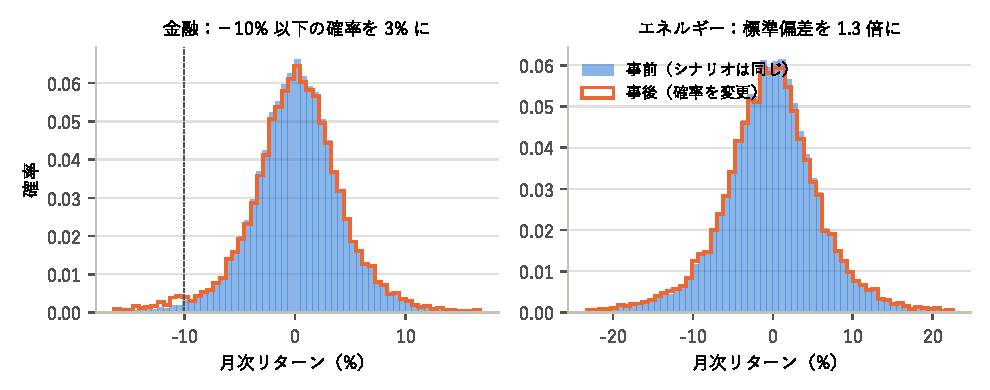
\includegraphics[width=0.95\linewidth]{fig_ep.pdf}
\caption{同じシナリオの、事前の確率（塗り）と事後の確率（線）。左：金融の $-10\%$ 以下の確率を上げると、左の裾の確率が増える。右：エネルギーの標準偏差を上げると、両方の裾の確率が増える。}
\label{fig:ep}
\end{figure}

結果は次のとおりである（\tabref{tab:ep}、\figref{fig:ep}）。

\begin{itemize}
\item 3 つのビューはすべて満たされた。情報技術と公益の差は \V{ep.spread1}\%、金融の下落の確率は \V{ep.tail1}\%、エネルギーの標準偏差は \V{ep.sdE1}\% になった。
\item ビューのない資産の分布も動く。金融の下落の確率を上げると、金融と一緒に下がりやすいシナリオの確率が上がるので、ほとんどのセクターで下落の確率が上がり、平均が下がる。一方、情報技術を押し上げる順位のビューの影響で、情報技術と連動しやすい資本財は平均が上がった。相関の構造は、シナリオを通じてそのまま保たれる。
\item 相対エントロピーは \V{ep.kl}、確率の偏りを表す有効なシナリオの割合（$\exp(-\sum q\log q)/J$）は \V{ep.ens}\% で、確率の変え方は穏やかだった。
\item 確信度 $c=0.5$ で混ぜると、差は \V{ep.c.spread}\%、下落の確率は \V{ep.c.tail}\% になる。
\end{itemize}

\section{平均のビューなら、BL とほぼ同じ}

ビュー 1 を「差がちょうど 1\%」という等式にして、それだけを入れると、エントロピー・プーリングによる平均の変化は、市場版の BL を $\Omega\to0$ で使ったときの変化と、最大 \V{ep.maxdiff}\% の差で一致した（\tabref{tab:ep} の右の 2 列）。

Meucci は、正規分布の市場に線形の平均のビューを入れる場合、エントロピー・プーリングが BL の結果を再現することを示している。今回の事前分布は $t$ 分布だが、平均の条件付けは楕円形の分布ならほぼ同じ形になる。エントロピー・プーリングは BL を置き換えるものではなく、BL を含む広い枠組みである。違いが出るのは、順位、ボラティリティ、裾の確率のような、平均以外のビューを入れたときである。

\section{使うときの注意}

\begin{itemize}
\item \textbf{シナリオの数}：裾のビュー（下落の確率など）は、裾に十分なシナリオがないと満たせないか、少数のシナリオに確率が集中する。有効なシナリオの割合が小さくなったら、シナリオを増やすか、ビューを弱める。
\item \textbf{満たせないビュー}：シナリオの範囲の外のビュー（すべてのシナリオで $-5\%$ より上なのに、「$-10\%$ 以下の確率は 3\%」）は満たせない。双対の解が発散したら、まずこれを疑う。
\item \textbf{不確かさの扱い}：エントロピー・プーリングのビューは、それ自体には不確かさを持たない（満たすか満たさないか）。不確かさは、式~\eqref{eq:ep-pool} の確信度 $c$ で入れる。$c$ も、当たり具合から決めるのが望ましい（\chapref{ch:accuracy}）。
\item \textbf{確率の変化を見る}：事後の確率 $q/p$ の分布を見て、一部のシナリオに極端な重みが付いていないかを確かめる。
\end{itemize}

\begin{tipbox}[コツ：エントロピー・プーリング]
\begin{enumerate}
\item 平均のビューだけなら、BL で十分である。順位、ボラティリティ、裾の確率、相関のビューを入れたいときに使う。
\item 事前のシナリオは、裾の厚さを表せるもの（過去のリターン、$t$ 分布、GARCH のシミュレーション）にする。
\item ビューの不確かさは、確信度 $c$ で事前と事後を混ぜて入れる。
\item 有効なシナリオの割合を確かめ、確率が一部に集中していないかを見る。
\end{enumerate}
\end{tipbox}

\begin{keybox}[この章のまとめ]
\begin{itemize}
\item エントロピー・プーリングは、シナリオの値を変えずに確率だけを変え、ビューを満たす中で事前にいちばん近い（相対エントロピーが最小の）分布を選ぶ。
\item 双対で解けば、条件の数だけの小さな凸の問題になる。事後の確率は、事前の確率に条件の式の指数を掛けたものになる。
\item 順位・ボラティリティ・裾の確率のビューを、裾の厚い分布に入れられる。平均のビューだけなら、BL とほぼ同じ答えになる。
\end{itemize}
\end{keybox}
